%%%%%%%%%%%%%%%%%%%%%%%%PREAMBLE%%%%%%%%%%%%%%%%%%%%%%%%%%%%%%%%%%%%
\documentclass[10pt]{beamer} 
\usetheme[height=7mm]{Rochester} 
\usecolortheme[named=blue]{structure}
\useoutertheme{shadow}
\useinnertheme{rounded}

\setbeamertemplate{items}[ball]
\setbeamertemplate{blocks}[rounded][shadow=true]
\setbeamertemplate{navigation symbols}{}

%%%%%%%%%%%%%%%%%%%%%%%%PACKAGES%%%%%%%%%%%%%%%%%%%%%%%%%%%%%%%%%%%%
\usepackage{amsfonts,amssymb,amsmath,bm}
\usepackage{epstopdf}
\usepackage{pdfpages}
\usepackage{setspace}
\usepackage{lscape}
\usepackage{graphicx}
\usepackage{subfig,graphicx}
\usepackage{caption}
\usepackage{multimedia}
\usepackage{media9}


%%%%%%%%%%%%%%%%%%%%%%%%DEFINITIONS%%%%%%%%%%%%%%%%%%%%%%%%%%%%%%%%%
\input{/Users/daniele/Dropbox/Career/Research/MyPapers/definitions.tex}
\def \orthmat{\Matrix{W}}							%orthogonal matrix


%%%%%%%%%%%%%%%%%%%%%%%%TITLE%%%%%%%%%%%%%%%%%%%%%%%%%%%%%%%%%

\title[The Reproducible Research Repository]{The Reproducible Research Repository: \\ Open innovation in the Digital Music Research Community}
\author[Barchiesi et al.]{Daniele Barchiesi, Luis Figueira, Chris Cannam and Mark D. Plumbley}
\institute[C4DM]{
  Centre for Digital Music\\
  School of Electronic Engineering and Computer Science\\
  Queen Mary University of London\\[2ex]
  \texttt{name.surname@eecs.qmul.ac.uk}\\
\titlegraphic{\includegraphics[width=1.5cm]{images/c4dmLogo.pdf}}
\titlegraphic{\includegraphics[width=1.5cm]{images/qmLogo.pdf}}
}
\date[17 Dec. 2013]{17 Dec. 2013 - DMRN+8}
\begin{document}

\maketitle

\begin{frame}{Overview}
\begin{block}{}
\begin{itemize}
\item Reproducible research
\item The reproducible research repository: background and motivations
\item rrr.soundsoftware.co.uk: A reproducible research repository for the digital music research community
\item A quick live demo
\item Question time...
\end{itemize}
\end{block}
\end{frame}

\begin{frame}{The Research Lifecycle}
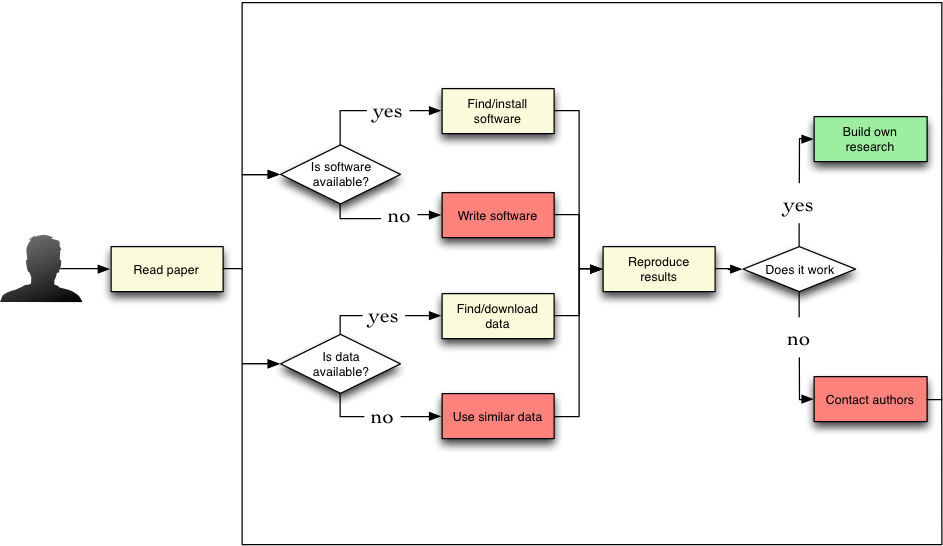
\includegraphics[width=\linewidth]{./images/research-lifecycle.jpg}
\end{frame}

\begin{frame}{What is wrong with research results?}
\begin{block}{Many results in digital music are not reproducible}
\begin{itemize}
\item 82\% of research develop software
\begin{itemize}
\item 39\% of those took steps to make their code reproducible
\begin{itemize}
\item 35\% of those published their code
\end{itemize}
\end{itemize}
\item \textbf{11\%} of researchers published reproducible research code
\end{itemize}
\end{block}
\begin{block}{The validity of unreproducible research can be questionable}
\begin{itemize}
\item Lack of statistical rigor can lead to misleading results: \emph{fooled by randomness}
\item Lack of career incentives can lead to publication bias: \emph{only positive results appear in journals}
\end{itemize}
\end{block}
\end{frame}

\begin{frame}{The soundsoftware project}
\begin{block}{Promoting reproducible research}
\begin{itemize}
\item Reproducible research prizes (AES conf. on Semantic Audio)
\item Workshops on software carpentry
\item Software repository: \url{http://code.soundsoftware.ac.uk}
\item Reproducible Research Repository (RRR) \url{http://rrr.soundsoftware.ac.uk}
\end{itemize}
\end{block}

The Reproducible Research Repository lowers the barriers for reproducible research by enabling sharing of resources and workflows
\end{frame}

\begin{frame}{The reproducible research repository}
\begin{block}{}
\begin{itemize}
\item Organised around \textbf{experiments}: self-contained units corresponding to figures and tables present in academic publications
\item Each experiment is linked to a number of \textbf{resources} 
\begin{itemize}
\item Datasets
\item Software
\item Publications
\end{itemize}
\item Each experiment contains \textbf{instructions} on how to reproduce results, including
\begin{itemize}
\item Software versions and parameters
\item Description of workflows
\end{itemize}
\end{itemize}
\end{block}
\end{frame}

\begin{frame}{Reproducible research is reproducible}
\begin{block}{The reproducible Research Repository}
\begin{itemize}
\item RRR has been designed using Drupal, the biblio module and various other customizations
\item Go to \url{https://code.soundsoftware.ac.uk/projects/rr-repo/wiki/How_to_create_RRR_from_scratch} to find the instructions on how to recreate RRR
\end{itemize}
\end{block}
\begin{block}{This presentation}
\begin{itemize}
\item Go to \url{https://github.com/danieleb/rrr_presentation} to download it
\end{itemize}
\end{block}
\end{frame}
\end{document}